

\chapter{Introduction}
The Large Hadron Collider (LHC) is a particle accelerator at CERN, the European Organization for Nuclear Research, near Geneva, Switzerland. It was developed and designed primarily to explore the physics beyond the Standard Model (BSM), including searches for dark matter, CP violation, new particles, and supersymmetry. \cite{Nath_2010} One of its main discoveries was the Higgs boson, which was confirmed in 2012 by the Compact Muon Solenoid (CMS) and A Toroidal LHC Apparatus (ATLAS) experiments, almost simultaneously and independently \cite{Aad_2012, Chatrchyan_2012}, both of which are general-purpose detectors within the LHC. The discovery provided a fundamental understanding of how particles acquire mass through the electroweak symmetry breaking mechanism, laying the foundation for a new era in particle physics. \cite{Pich_2016}

However, there are still a lot of open questions, most of which require increasing the probability of rare processes. One study focused on this task and observed that the cross-section, or the likelihood of rare processes, increases with higher center-of-mass energies (see Figure \ref{fig:crosssection}). \cite{cartiglia2013measurementprotonprotontotalelastic} Therefore, the CMS detector requires upgrades to address this challenge. Instead of solely relying on higher energies, the focus of the High-Luminosity LHC (HL-LHC) will be on increasing luminosity, or the number of collisions per unit time, by a factor of 5 compared to current conditions. \cite{atlas2019reportphysicshllhcperspectives} This opens up new possibilities for future discoveries in the search for BSM physics.

\begin{figure}[h]
    \centering
    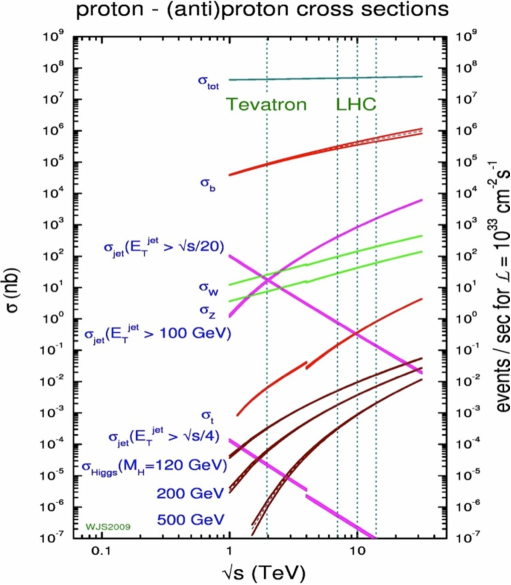
\includegraphics[width=0.55\textwidth]{images/cross-sections.png}
    \caption{Cross-sections for different processes at various collision energies as a function of center-of-mass energy \( \sqrt{s} \) \cite{cartiglia2013measurementprotonprotontotalelastic}.}
    \label{fig:crosssection}
\end{figure}

Central to particle tracking in the CMS Phase-2 upgrade detector is the Inner Tracker (IT) which will face enormous operational challenges as an extreme radiational exposure with a neutron equivalent fluence of up to $2.3 \times 10^{16}\text{n}_{eq}/\text{cm}^{2}$, a total ionizing dose (TID) reaching approximately $12\text{MGy}$ ($1.2 \text{Grad}$), and pixel hit rates as high as $3\text{GHz/cm}^{2}$ with up to 200 collisions per bunch crossing \cite{Apollinari:2284929, Malik:2816244}. To operate effectively under these harsh conditions, the upgraded detector must have improved spatial resolution, achieved through the reduced pixel size and sensor thickness, and electronics capable of high rates and enhanced radiation tolerance. The CMS Phase-2 upgrade is currently under development and testing at various international facilities, including Fermi National Accelerator Laboratory (FNAL), CERN, and German Electron Synchotron (DESY), to validate these technological advancements and ensure their robustness for HL-LHC operation.

At the FNAL Testbeam studies, silicon pixel sensors used as the Device Under Test (DUT) have been characterized in terms of cluster size and spatial resolution in the non-irradiated case. The pixel telescope resolution is utilized as the reference frame in determining the DUT resolution is approximately $10~\mu\text{m}$ and is attained through the integration of several layers of pixel planes.

When a charged particle traverses a silicon pixel sensor, it deposits energy and generates electron-hole pairs, following a Landau-like distribution in charge. In particular, particles that produce significantly higher than average charge are often associated with secondary interactions, such as delta-rays, which can complicate the reconstruction of the original particle trajectory. For this reason, it is relevant to study the pixel resolution, cluster size, and crosstalk as a function of the charge bins within the Landau distribution.

These studies not only provide a deeper understanding of sensor performance but also support a slight improvement of the telescope's resolution and allow for a more accurate determination of the DUT resolution. Chapters~3, 5 presents and discusses these investigations in detail.

Moreover, The HL-LHC upgrade will enhance the complexity and event rates, leading to a 7.5-fold rise in the readout rate \cite{Fernandez_Perez_Tomei_2020}. Currently, at the CMS experiment, event selection for further analysis is manually determined based on detector performance, particularly tracking. However, with the upgrade, the number of monitoring elements (MEs) will grow substantially, making manual decision-making both labor-intensive and prone to bias. Therefore, some automated tools capable of detecting unexpected or anomalous behavior will be highly beneficial. For this purpose, a Non-Negative Matrix Factorization (NMF) machine learning (ML) model is being explored as a possible approach. NMF enables dimensionality reduction of the input data to capture underlying patterns across Monitoring Elements (MEs), while reducing the reliance on manual inspection. So far, the model has been shown to successfully identify anomalies in synthetically generated data for one of the MEs. Chapters~4, 5 present and discuss this approach in detail.
